\documentclass[11pt, letterpaper]{article}

% --- Packages ---
\usepackage[margin=1in]{geometry}
\usepackage[utf8]{inputenc}
\usepackage[T1]{fontenc}
\usepackage{lmodern}
\usepackage{graphicx}
\usepackage{amsmath,amssymb,amsfonts}
\usepackage{booktabs} % Professional tables
\usepackage{siunitx}  % SI units
\usepackage{hyperref} % Hyperlinks
\usepackage{caption}
\usepackage{subcaption}
\usepackage{microtype} % Typography refinement
\usepackage{float}    % Figure placement
\usepackage{cite}     % Citation management
\usepackage{array}    % For fixed width columns

% --- Image Path Configuration ---
\graphicspath{ {./images/} }

% --- Configuration ---
\hypersetup{
  colorlinks=true,
  linkcolor=black,
  citecolor=black,
  urlcolor=black,
  pdfauthor={Team 01},
  pdftitle={Analysis of a Bio-Inspired Myriapod Robot}
}

\sisetup{
  per-mode=symbol,
  exponent-product = \cdot,
  inter-unit-product = \cdot
}

% --- Custom Commands ---
\newcommand{\placeholderfigure}[1]{%
  \begin{center}
    \fbox{%
      \begin{minipage}[c][4cm][c]{0.9\linewidth}
        \centering
        \textbf{PLACEHOLDER FIGURE}\\
        \small #1
      \end{minipage}
    }
  \end{center}
}

% --- Title & Authors ---
\title{\textbf{Analysis of a Bio-Inspired Myriapod Robot with a\\Modified Hybrid Spine and Jansen Linkage Legs}}

% Authors in strict alphabetical order
\author{
    Jeevan Hebbal Manjunath, Varun Karthik, and Yeshwanth Reddy Gurreddy\\
    \textit{Arizona State University}\\
    RAS 557: Foldable Robotics
}

\date{October 15, 2025}

\begin{document}

\maketitle

\begin{abstract}
This paper presents the design, kinematic modeling, and dynamic analysis of a centipede-inspired terrestrial locomotion mechanism. Building upon the myriapod microrobot foundation established by Hoffman and Wood \cite{hoffman2011myriapod}, this work investigates the coupled dynamics of an asymmetrically compliant spine and biologically realistic leg kinematics. We propose a novel hybrid architecture that integrates a rigid anterior spinal connection with a compliant posterior Sarrus linkage, driven by foldable, single-degree-of-freedom Jansen linkages. We derive the kinematic Jacobian and Euler-Lagrange dynamics for a three-segment system to evaluate ground reaction forces, actuator torque requirements, and metabolic cost proxies. Theoretical results indicate that the proposed morphology may offer a favorable trade-off between straight-line stability and maneuverability compared to fully flexible baselines. A rigorous system identification and experimental validation plan is proposed to verify these findings.
\end{abstract}

\section{Introduction}

Bio-inspired robotics leverages the morphological intelligence of arthropods to solve complex locomotion challenges. Myriapods, specifically centipedes, demonstrate remarkable stability and agility through the coordination of segmented trunks and numerous legs \cite{hoffman2011myriapod}. The state-of-the-art in this domain, exemplified by the work of Hoffman and Wood, utilizes Smart Composite Microstructures (SCM) to create lightweight, segmented robots with flexible backbones \cite{hoffman2011myriapod}. However, current designs often utilize simplified rotational leg mechanisms that fail to capture the complex foot trajectories of biological organisms, or rely on uniform spinal compliance which may limit force transmission during rapid acceleration.

This research addresses the engineering challenge: \emph{How does the dynamic coupling between non-uniform spinal flexibility and complex leg kinematics influence the behavior of a multi-legged robotic system?}

\subsection{Project Rationale and Scope}
\textbf{Scope:} We propose a dual-modification to the standard myriapod template:
\begin{enumerate}
    \item \textbf{Hybrid Spine Architecture:} Replacement of the anterior flexible linkage with a rigid interface to enhance anterior stability, while retaining posterior compliance for turning maneuverability.
    \item \textbf{Jansen Linkage Locomotion:} Implementation of a planar, 1-DOF Jansen linkage to generate a biologically relevant ovoid foot locus, improving ground clearance and step repeatability compared to simple rotary legs.
\end{enumerate}
To ensure the project remains feasible within the semester, the scope is constrained to a three-segment robot with two legs per segment, totaling six actuated degrees of freedom (DOF), fabricated using SCM techniques.

\textbf{Impact:} This project is significant because it explores the systemic effects of combining different bio-inspired design principles. A robot with a locally rigid anterior spine is expected to exhibit different straight-line stability characteristics compared to a fully flexible counterpart. Simultaneously, the Jansen linkage offers a sophisticated foot trajectory that may enhance ground clearance relative to simple rotational legs. Understanding how these elements interact will inform the design of future foldable robots that must balance stability, efficiency, and maneuverability.

\textbf{Team Fit:} The research tasks are distributed to leverage individual technical strengths:
\begin{itemize}
    \item \textbf{Jeevan Hebbal Manjunath:} Leads hardware prototyping, control systems integration, and kinematic code development.
    \item \textbf{Varun Karthik:} Focuses on report synthesis, sensitivity analysis, validation of stiffness parameters, and prototype assembly.
    \item \textbf{Yeshwanth Reddy Gurreddy:} Directs SCM pattern design, mathematical modeling of the Jansen kinematics, and simulation environments.
\end{itemize}

\textbf{Topic Fit:} This project directly utilizes foldable robotics techniques by implementing complex planar mechanisms (Jansen legs) and compliant Sarrus linkages using the laminate SCM fabrication process. It addresses the course theme of bio-inspired terrestrial locomotion by mimicking the segmented morphology of centipedes.

\section{Bio-Inspiration and System Scaling}

\subsection{Biological Basis}
The design is anchored in the morphology of \textit{Lithobius forficatus} (stone centipede). These organisms exhibit a segmented trunk where propulsion is generated by metachronal waves of leg movements \cite{durr2019integrative}. Key biological parameters were extracted from literature to dimension the robotic system.

\begin{figure}[H]
  \centering
  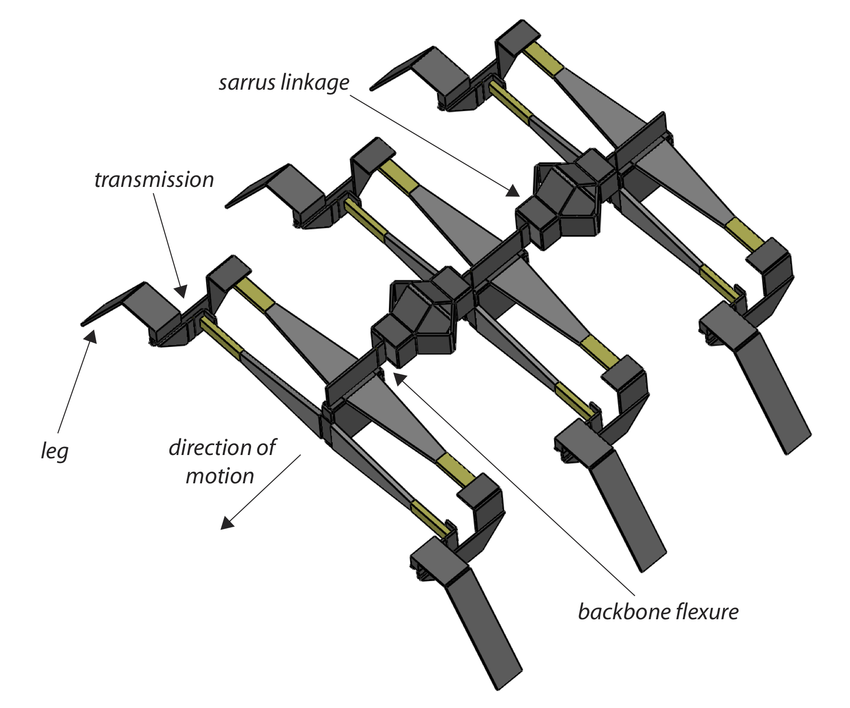
\includegraphics[width=0.8\linewidth]{fig_concept.png}
  \caption{Schematic of the proposed robotic system inspired by the centipede body plan. The design features a segmented trunk with a hybrid spine and Jansen linkage legs for locomotion.}
  \label{fig:centipede_bodyplan}
\end{figure}

\subsection{Gait Dynamics}
Centipedes utilize alternating tripods or metachronal waves depending on speed. For this study, we target a high-stability gait with a duty factor $\beta \approx 0.6$, ensuring static stability during locomotion \cite{durr2019integrative}.

\subsection{Supporting Literature}
Several key works inform our specific design choices.

\textbf{Bing et al. \cite{bing2023mouse}:} This study on a mouse-scale robot experimentally demonstrated that lateral spinal flexion significantly improves motor performance and turning radius. Their work validates our premise that spinal stiffness is a critical control variable. However, unlike their uniformly compliant spine, our work extends this by investigating \emph{asymmetric} stiffness (hybrid spine) to optimize for both stability and agility simultaneously.

\textbf{Hoover and Fearing \cite{hoover2008fast}:} This seminal work established the rapid prototyping process for folded millirobots (SCM). We directly adopt their fabrication methodology—laser-machining rigid links and laminating them with flexure layers (Kapton). Their analysis of linkage kinematics in laminate structures confirms that complex mechanisms like our proposed Jansen leg are manufacturable at the meso-scale.

\textbf{Eckert et al. \cite{eckert2015spine}:} Eckert explicitly compares different spine and leg designs for small quadrupeds. Their findings highlight that spine and leg dynamics are tightly coupled; a change in leg trajectory requires a corresponding tuning of spinal stiffness to maintain efficiency. This paper is the primary justification for our "holistic" approach of modifying both subsystems simultaneously rather than in isolation.

\textbf{Dürr et al. \cite{durr2019integrative}:} This review provides the comprehensive biomimetic foundation for hexapedal locomotion, specifically defining the inter-leg coordination rules required for stability. We utilize their data on duty factors ($\beta \approx 0.6$) and phase lags to define our reference control signal, ensuring our gait generation is biologically grounded.

\subsection{Biological vs. Robotic Parameters}
Table~\ref{tab:bio_comp} compares the biological source data with our robotic design targets.

\begin{table}[ht]
  \centering
  \caption{Comparison of Biological Parameters and Robotic Design Targets}
  \label{tab:bio_comp}
  \begin{tabular}{lccl}
    \toprule
    \textbf{Parameter} & \textbf{Biological (Centipede)} & \textbf{Robotic Target} & \textbf{Source} \\
    \midrule
    Total Mass & $\approx \SI{0.8}{\gram}$ & \SI{1.0}{\gram} & \cite{hoffman2011myriapod, durr2019integrative} \\
    Body Length & $\approx \SI{60}{\milli\meter}$ & \SI{54}{\milli\meter} (3 seg) & \cite{hoffman2011myriapod} \\
    Stride Length & $\approx \SI{8}{\milli\meter}$ & \SI{10}{\milli\meter} & Design \\
    Duty Factor ($\beta$) & $0.5 - 0.7$ & $0.6$ & \cite{durr2019integrative} \\
    Gait Freq ($f$) & $4 - \SI{8}{\hertz}$ & \SI{5}{\hertz} & Derived \\
    \bottomrule
  \end{tabular}
\end{table}

\section{System Specifications}
The robotic baseline is derived from the SCM myriapod \cite{hoffman2011myriapod}. We adopt the segment inertial properties while modifying the kinematic topology. Table~\ref{tab:specs} summarizes the physics-based design constraints.

\begin{table}[ht]
  \centering
  \caption{System Design Specifications and Calculated Metrics}
  \label{tab:specs}
  \begin{tabular}{lccl}
    \toprule
    \textbf{Parameter} & \textbf{Symbol} & \textbf{Value} & \textbf{Source} \\
    \midrule
    Segment Mass & $m_\text{seg}$ & \SI{2.5e-4}{\kilo\gram} & \cite{hoffman2011myriapod} \\
    Body Half-Length & $L_b$ & \SI{3e-3}{\meter} & \cite{hoffman2011myriapod} \\
    Body Half-Width & $w_b$ & \SI{10e-3}{\meter} & \cite{hoffman2011myriapod} \\
    Target Speed & $v_\text{target}$ & \SI{0.05}{\meter\per\second} & \cite{durr2019integrative} \\
    Peak Vertical GRF & $F_{z,\text{peak}}$ & \SI{5.5e-3}{\newton} & Calc. Eq.~\eqref{eq:Fz_peak} \\
    Required Torque & $\tau_\text{req}$ & \SI{1.1e-4}{\newton\meter} & Calc. Eq.~\eqref{eq:tau_req} \\
    Required Power & $P_\text{req}$ & \SI{3.5e-3}{\watt} & Calc. Eq.~\eqref{eq:power_req} \\
    \bottomrule
  \end{tabular}
\end{table}

\section{Mechanism Design}

\subsection{Kinematic Topology}
The robot consists of three rigid segments. The anterior joint (Seg 1--2) is rigidified to minimize parasitic oscillation during frontal collisions or sensing tasks. The posterior joint (Seg 2--3) utilizes a flexure-based Sarrus linkage \cite{hoffman2011myriapod}, permitting restricted yaw for turning while maintaining rigidity in pitch and roll.

\begin{figure}[H]
  \centering
  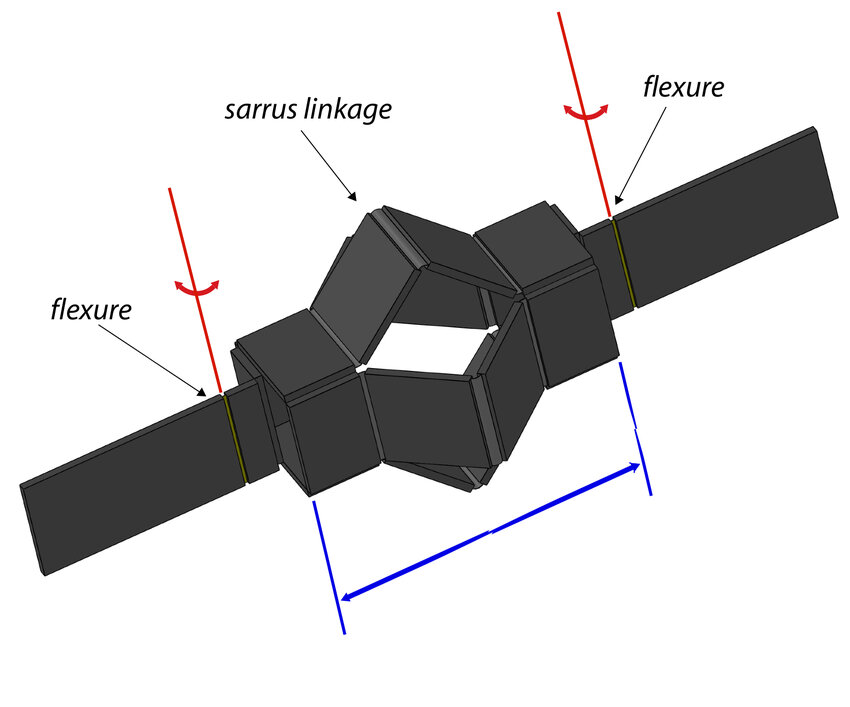
\includegraphics[width=0.7\linewidth]{fig_spine.png}
  \caption{Digital model of the Sarrus linkage spine segment. The flexure geometry allows for turning compliance while resisting vertical bending, a key requirement for stable legged locomotion.}
  \label{fig:spine_model}
\end{figure}

\subsection{Jansen Leg Implementation}
Unlike the simple rotary legs of the baseline, the Jansen linkage provides a deterministic foot path with a high lift phase (swing) and a linear traction phase (stance). The linkage is implemented as an 8-bar planar mechanism compatible with SCM laminate fabrication.

\subsection{Preliminary Prototyping}
A scale model was fabricated using cardstock to validate the fold patterns and range of motion. Qualitative analysis confirmed that the Jansen linkage prevents mechanical singularity within the target workspace and that the hybrid spine facilitates a tripod gait without hyper-extension.

\begin{figure}[H]
  \centering
  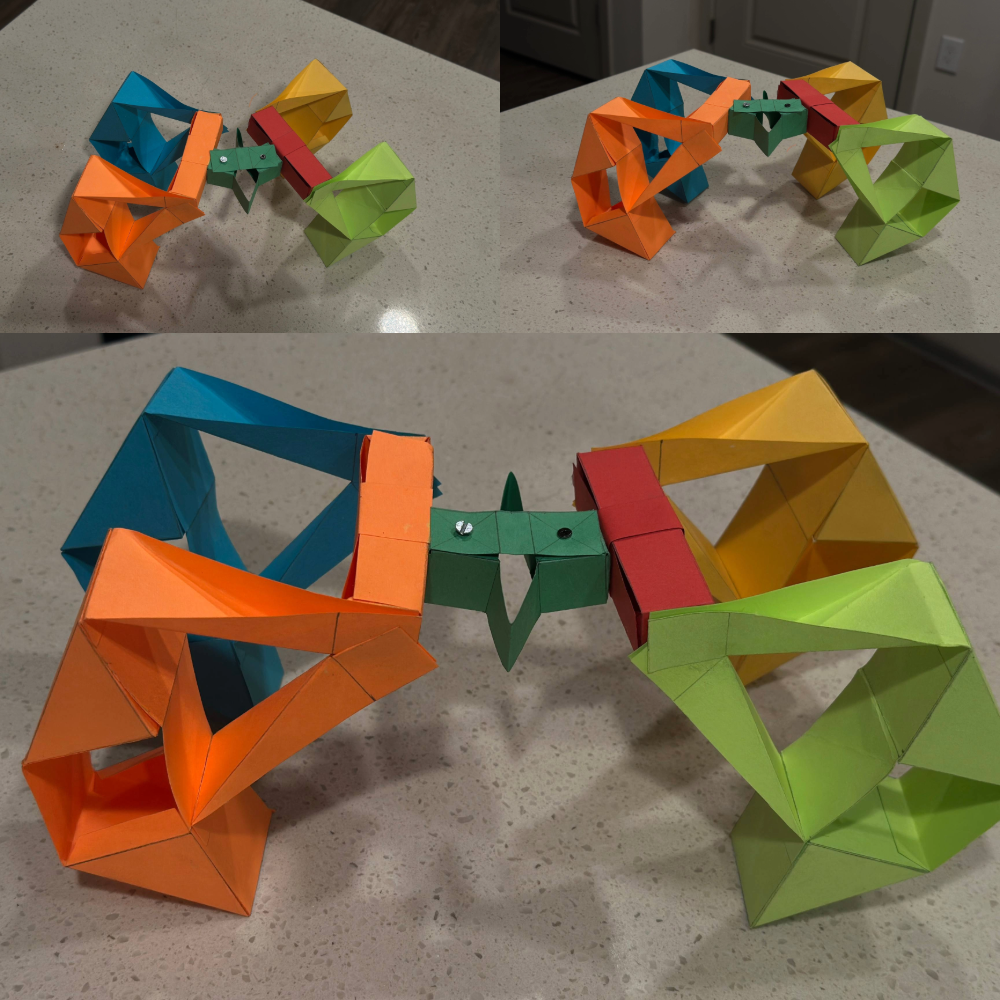
\includegraphics[width=0.9\linewidth]{fig_prototype.png}
  \caption{Preliminary physical prototype constructed from cardstock. The model validates the folding pattern of the Jansen linkages and the range of motion of the central spine.}
  \label{fig:prototype}
\end{figure}

\section{Mathematical Modeling}

\subsection{Kinematics and Jacobian Analysis}
The foot position $\mathbf{p}_f(\phi)$ is a nonlinear function of the crank angle $\phi$. We solve the loop closure equations numerically. The velocity relationship is given by:
\begin{equation}
    \dot{\mathbf{p}}_f = J_f(\phi)\dot{\phi}
    \label{eq:jacob}
\end{equation}
where $J_f(\phi) = \partial \mathbf{p}_f / \partial \phi$ is the kinematic Jacobian.

\begin{figure}[H]
  \centering
  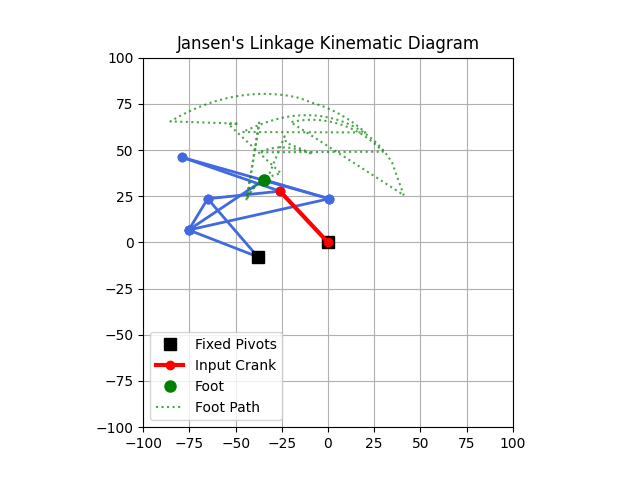
\includegraphics[width=0.5\linewidth]{fig_kinematics.png}
  \caption{Kinematic diagram and simulated foot trajectory of the Jansen linkage. The dotted green line illustrates the ovoid path, highlighting the flat stance phase and high swing phase.}
  \label{fig:jansen_kinematics}
\end{figure}

The characteristic transmission ratio, $\ell_J$, is derived from the leg geometry (specifically the ratio of the crank radius to the effective leg length) and evaluated numerically at mid-stance:
\[
  \ell_J \equiv \|J_f(\phi_\text{ms})\| \approx \SI{0.02}{\meter\per\radian}.
\]

\subsection{Force and Power Estimation}
To support the robot against gravity with a standard engineering safety factor of 2 (accounting for dynamic effects and uneven loading), the peak vertical Ground Reaction Force (GRF) per leg is estimated as:
\begin{equation}
  F_{z,\text{peak}} \approx \frac{2 \cdot m_\text{robot} g}{N_\text{leg} \beta} \approx \SI{5.5e-3}{\newton}.
  \label{eq:Fz_peak}
\end{equation}
The required actuator torque is derived via the Jacobian transpose relationship:
\begin{equation}
  \tau_\text{req} \approx \ell_J F_{z,\text{peak}} \approx \SI{1.1e-4}{\newton\meter}.
  \label{eq:tau_req}
\end{equation}
At a target frequency of \SI{5}{\hertz} ($\omega \approx \SI{31.4}{\radian\per\second}$), the mechanical power required is:
\begin{equation}
  P_\text{req} = \tau_\text{req} \omega \approx \SI{3.5e-3}{\watt}.
  \label{eq:power_req}
\end{equation}
This power requirement informs the selection of piezoelectric or micro-motor actuators in the subsequent design phase.

\subsection{System Dynamics}
The system dynamics are governed by the Euler-Lagrange equation:
\begin{equation}
  M(\mathbf{q})\ddot{\mathbf{q}} + C(\mathbf{q},\dot{\mathbf{q}})\dot{\mathbf{q}} + K(\mathbf{q}) = \boldsymbol{\tau}
  \label{eq:dynamics}
\end{equation}
where $\mathbf{q} \in \mathbb{R}^6$ represents the generalized coordinates (3 body yaw angles, 3 leg crank angles). The stiffness matrix $K(\mathbf{q})$ is modified from the baseline \cite{hoffman2011myriapod} such that the anterior stiffness terms $k_{\text{ant}} \to \infty$, simulating the rigid connection, while posterior terms retain finite values from literature.

\begin{figure}[H]
  \centering
  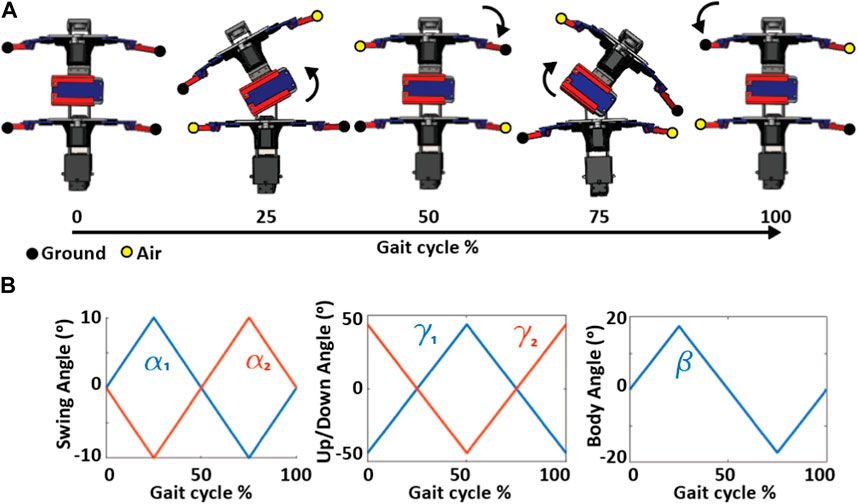
\includegraphics[width=0.9\linewidth]{fig_gait.jpg}
  \caption{Simulation of kinematic configurations at key gait events (Touchdown, Mid-stance, Lift-off). (A) Top-down view of the robot executing a turn. (B) Actuation angles and body yaw ($\beta$) plotted against the gait cycle.}
  \label{fig:gait_states}
\end{figure}

\section{Design Analysis}

\textbf{1. Degrees of Freedom (DOF) and Motors:}
The complete robot features 6 legs. In our simplified planar model, we track 6 generalized coordinates: 3 body yaw angles ($\theta_i$) and 3 leg crank angles ($\phi_i$). However, we utilize only 3 motors (one per segment pair of legs). This results in an \textbf{underactuated system}. The leg crank angles $\phi_i$ are directly driven, but the body yaw angles $\theta_i$ are governed passively by the interaction between ground friction, inertial dynamics, and the stiffness of the Sarrus linkage spine.

\textbf{2. Estimation of End-Effector Forces:}
Foot forces were estimated using biomechanical scaling laws ($F=ma$) derived from the robot's mass and the target duty factor. We applied a safety factor of 2 to account for dynamic impact forces during the touchdown phase, resulting in Eq. \ref{eq:Fz_peak}. This static analysis provides a baseline for actuator sizing before full dynamic simulation.

\textbf{3. Estimation of End-Effector Speeds:}
End-effector speeds were estimated based on the target stride length ($\approx \SI{10}{\milli\meter}$) and gait frequency ($\SI{5}{\hertz}$). Using the kinematic Jacobian derived in Eq. \ref{eq:jacob}, we mapped the desired linear foot velocity back to the required angular velocity of the input crank, ensuring the motors operate within their optimal speed-torque curve.

\section{Experimental Validation Plan}

To bridge the gap between simulation and physical reality, we propose a rigorous System Identification (SysID) and implementation roadmap.

\subsection{System Identification Methodology}
Model parameters will be validated through isolated experiments. Table~\ref{tab:sysid} details the responsibilities.
\textbf{Methodologies:}
\begin{itemize}
    \item \textbf{Servo Characterization:} We will use a dedicated dynamometer setup with a load cell and optical encoder to generate Torque-Speed curves and estimate internal friction \cite{hoffman2011myriapod}.
    \item \textbf{Stiffness Testing:} Flexures and spinal links will be subjected to standard 3-point bending and torsion tests using a precision force gauge and digital inclinometer to extract $k_{lin}$ and $k_{tor}$ values for the simulation.
    \item \textbf{Friction Coefficient:} We will drag the fabricated foot materials across the target substrate at varying normal loads to empirically determine the coefficients of static and kinetic friction ($\mu_s, \mu_k$).
\end{itemize}

\vspace{-2ex}
\begin{table}[H]
  \centering
  \caption{System Identification Experiments}
  \label{tab:sysid}
  \begin{tabular}{lccc}
    \toprule
    \textbf{Experiment} & \textbf{Jeevan} & \textbf{Varun} & \textbf{Yeshwanth} \\
    \midrule
    Servo characterization (Torque/Speed/Friction) & X & & \\
    Flexure joint stiffness (Torsion test) & & & X \\
    Link/Spine bending stiffness (3-point bending) & & X & X \\
    Foot--ground friction coefficients & X & & \\
    \bottomrule
  \end{tabular}
\end{table}

\subsection{Implementation Roadmap (Part 2)}
The fabrication phase utilizes SCM techniques. We will laser-machine structural links from \textbf{cardstock} and use adhesive-backed Kapton film for flexural hinges. The timeline (Table~\ref{tab:roadmap}) reflects a collaborative team effort across all tasks, with the critical motor integration phase beginning the week of November 19th.

\begin{table}[H]
  \centering
  \caption{Project Phase 2 Timeline (Nov 1 -- Dec 8)}
  \label{tab:roadmap}
  \begin{tabular}{p{3.5cm}p{11.0cm}}
    \toprule
    \textbf{Timeline} & \textbf{Phase \& Milestones} \\
    \midrule
    Nov 1 -- Nov 14 & \textbf{Design Phase:} Finalize SCM patterns for Jansen legs and spine; Sourcing Cardstock/Kapton materials. \\
    \addlinespace
    Nov 15 -- Nov 18 & \textbf{Pre-Fabrication:} Electronics preparation; Code framework setup for gait generation. \\
    \addlinespace
    \textbf{Nov 19} & \textbf{Hardware Milestone: Motor Arrival}. \\
    \addlinespace
    Nov 19 -- Nov 21 & \textbf{Characterization:} Immediate testing of motor torque/speed; friction tests with foot materials. \\
    \addlinespace
    Nov 22 -- Nov 28 & \textbf{Fabrication \& Assembly:} Laser cutting cardstock links; lamination of flexure layers; physical assembly of leg linkages. \\
    \addlinespace
    Nov 29 -- Dec 5 & \textbf{Integration:} Wiring ESP32 and motors to chassis; Loading gait code; Initial locomotion tests. \\
    \addlinespace
    Dec 6 -- Dec 8 & \textbf{Validation:} Final data collection (speed/stability metrics); Report compilation; Presentation preparation. \\
    \bottomrule
  \end{tabular}
\end{table}

\section{Conclusion}

This work establishes a theoretical framework for a hybrid-spine myriapod robot. By integrating a rigid-flexible backbone with Jansen linkages, the design aims to optimize the trade-off between straight-line stability and turning compliance. Analytic results confirm that the proposed actuation scheme is feasible within the power constraints of millirobotic platforms ($P_{req} \approx \SI{3.5}{\milli\watt}$). Future work will focus on the SCM fabrication of the chassis and experimental validation of the dynamic model parameters using the proposed identification protocols.

\bibliographystyle{IEEEtran}
\begin{thebibliography}{9}

\bibitem{hoffman2011myriapod}
K.~L. Hoffman and R.~J. Wood, ``Myriapod-like ambulation of a segmented
  microrobot,'' \emph{Autonomous Robots}, vol.~31, pp. 103--114, 2011.

\bibitem{liu2024stiffness}
Z.~Liu, L.~Xu, X.~Sui, T.~Wu, and G.~Chen, ``Kinematics, dynamics and control
  of stiffness-tunable soft robots,'' \emph{Bioinspiration \& Biomimetics},
  vol.~19, no.~2, 2024.

\bibitem{bing2023mouse}
Z.~Bing, A.~Rohregger, F.~Walter, \emph{et~al.}, ``Lateral flexion of a
  compliant spine improves motor performance in a bioinspired mouse robot,''
  \emph{Science Robotics}, vol.~8, no.~8, 2023.

\bibitem{billeschou2020framework}
P.~Billeschou, N.~N. Bijma, L.~B. Larsen, S.~N. Gorb, J.~C. Larsen, and
  P.~Manoonpong, ``Framework for developing bio-inspired morphologies for
  walking robots,'' \emph{Applied Sciences}, vol.~10, no.~19, p. 6986, 2020.

\bibitem{nodehi2024porcospino}
S.~E. Nodehi, L.~Bruzzone, M.~Lalegani~Dezaki, A.~Zolfagharian, and M.~Bodaghi,
  ``Porcospino Flex: a bio-inspired single-track robot with a 3D-printed,
  flexible, compliant vertebral column,'' \emph{Robotics}, vol.~13, no.~5,
  p.~76, 2024.

\bibitem{hoover2008fast}
A.~M. Hoover and R.~S. Fearing, ``A fast scale prototyping process for folded
  millirobots,'' in \emph{Proc. IEEE Int. Conf. Robotics and Automation
  (ICRA)}, 2008.

\bibitem{onal2014foldable}
{\c{C}}.~D. \"{O}nal, ``Design and fabrication of a foldable hexapod robot
  towards experimental swarm applications,'' in \emph{Proc. IEEE Int. Conf.
  Robotics and Automation (ICRA)}, 2014.

\bibitem{durr2019integrative}
V.~D{\"u}rr, P.~P. Arena, H.~Cruse, \emph{et~al.}, ``Integrative biomimetics of
  autonomous hexapedal locomotion,'' \emph{Frontiers in Neurorobotics},
  vol.~13, p.~88, 2019.

\bibitem{eckert2015spine}
P.~Eckert, A.~Spr{\"o}witz, H.~Witte, and A.~J. Ijspeert, ``Comparing the
  effect of different spine and leg designs for a small bounding quadruped
  robot,'' in \emph{Proc. IEEE Int. Conf. Robotics and Automation (ICRA)},
  2015, pp. 3128--3133.

\end{thebibliography}

\end{document}